% Chapter Template

\chapter{RESULTS \& DISCUSSION} % Main chapter title

\label{Results \& Discussion} % Change X to a consecutive number; for referencing this chapter elsewhere, use \ref{ChapterX}

\lhead{Chapter 4. \emph{Results \& Discussion}} % Change X to a consecutive number; this is for the header on each page - perhaps a shortened title

%----------------------------------------------------------------------------------------
%				SECTION 1
%----------------------------------------------------------------------------------------

\hspace{30} In   this   chapter,   we   present   and   discuss   the   results   obtained   from   our  
work.   We   explain   how   we   tested   the   different   geometric   properties   of   the  
heart­-shaped   primitive.   Without   loss   of   generality,   we   used   a   heart-­shaped  
object   centered   at   the   origin   (0,0,0), possesses   3   radial   vectors (5,0,0), (0,5,0) 
and (0,0,5) as   well   as   a   distance   to   cusps   of   4.   Let's   suppose   this  
object   called   \emph{amour}   and   is   stored   in   the   $heart\_example.g$   database. 
Given the situation of our work in the field of CAD, we   use   images   to   demonstrate   that 
  each   of   the   heart­-shape's   geometric  properties work.  

%----------------------------------------------------------------------------------------

\section{Type-in support for the heart­-shaped primitive}

\hspace{30} During   the   modeling   process,   a   designer   using   BRL­-CAD   creates objects   by   typing   
its   parameters   into   either   the   mged   or   archer   graphical   user  interfaces.   
Having   built   this   capacity   into   the   heart-­shaped   primitive,   we   used  
BRL-­CAD's \textbf{\textit{in}}[38] command to test its mettle.  

The   \textit{\textbf{in}}   command   enables   the   user   to   type   in   the   arguments   needed   to   create   a  shape   alongside   its   name   and   type.   It   supports   various   options   and   may   be  
invoked   with   no   arguments.   The   \textit{\textbf{-­s}}   option   invokes   the   primitive   edit   mode   on   a  
new   object   immediately   it   is   created.   In   order   to   test   the   type   in   support   of   the  
heart­-shaped   primitive,   we   create   the   \textit{amour}   object   by   typing   its   name,   type   and  
other   parameters   into   the   archer   interface.   After   opening   the   $heart\_example.g$  
database   database   destined   to   hold   the   \textit{amour}   object,   we   type   \textit{\textbf{“in   amour   hrt   0  
0   0   5   0   0   0   5   0   0   0   5   4”}}   into   archer's   command   line   interface.   The   object's  
name,   \textit{amour},   is   printed   on   the   command ­line   indicating   that   the   object   has  
indeed   been   created. Figure   4.1 below   shows   that   the   \textit{amour}  
heart-­shape object can be created by typing in its parameters through the keyboard.

\begin{figure}[htbp]
\centering
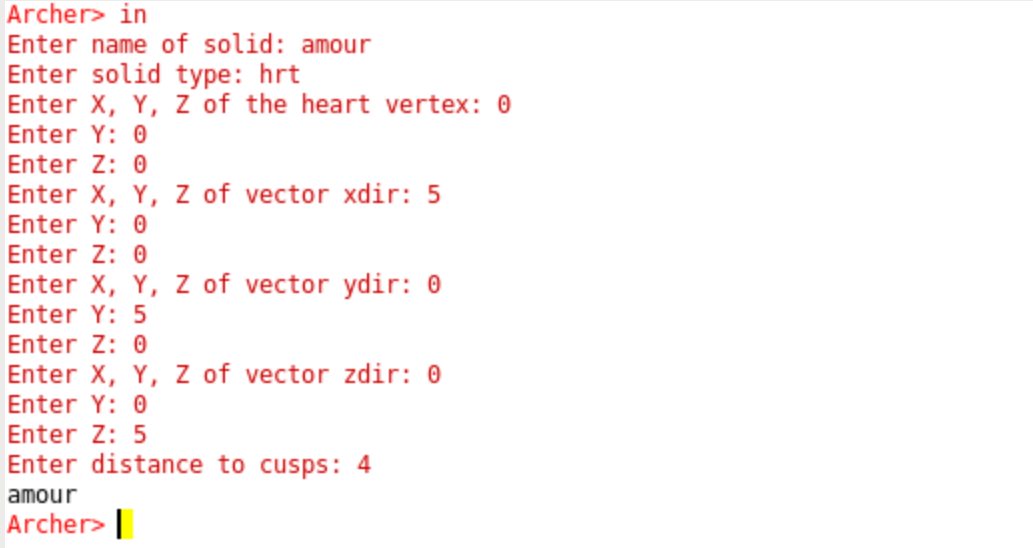
\includegraphics[trim=0.0cm 0.5cm 0.1cm 0.1cm, clip=true, totalheight=0.4\textheight]{Pictures/Typein.png}
\caption[Testing type in support for the heart-­shaped primitive in archer]{Testing type in support for the heart­-shaped primitive in archer}
\label{Typein}
\end{figure}

\clearpage

%----------------------------------------------------------------------------------------------------------------

%----------------------------------------------------------------------------------------------------------------
%						SECTION 2
%----------------------------------------------------------------------------------------------------------------
\section{Formatted description of the heart­-shaped primitive}

After   having   created   objects   for   modeling,   it   sometimes   becomes  
necessary   to   display   a   description   of   these   objects.   For   us   to   test   that   we   can  
describe   the   heart­shaped   primitive,   we   used   BRL-­CAD's   \textit{\textbf{l}}[39]   command   on  
the   amour   object.   The   \textit{\textbf{l (listing)}}   command   displays   a   verbose   description   of   a
 specific   list   of   objects.   If   the   shape   of   the   object   is   a   primitive,   then   detailed  
parameters   of   that   shape   are   displayed.   If   the   object   is   a   combination   of   other  
primitives,   then   the   boolean   formula   for   the   combination   is   listed   while   indicating  
any   accumulated   transformations.   If   a   shader   and   colour   has   been   assigned   to  
the   combination,   then   all   details   will   be   listed.   The   \textit{\textbf{-­t}}   (terse)   option   displays   a  
shorter list of primitive shape parameters.

\hspace{30} To   describe   the   \textit{amour}   object,   we   print   amour's   parameters   in   both   terse  
and   verbose   forms   by   running   the   \textit{\textbf{“l -t amour”}}   and   \textit{\textbf{“l amour”}}   commands  
respectively in the archer command prompt. This is shown in Figure 4.2 below.

\begin{figure}[htbp]
\centering
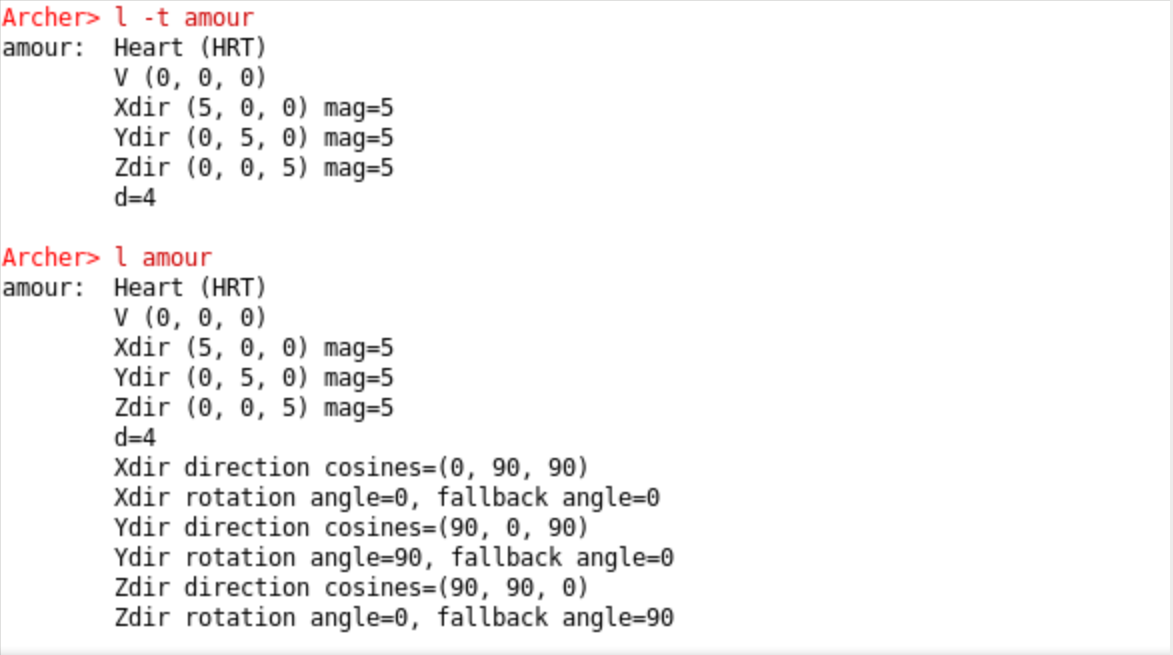
\includegraphics[trim=0.0cm 0.5cm 0.1cm 0.1cm, clip=true, totalheight=0.4\textheight]{Pictures/Describe.png}
\caption[Testing the formatted description of the heart­-shaped primitive]{Testing the formatted description of the heart­-shaped primitive}
\label{Describe}
\end{figure}

\clearpage

%-------------------------------------------------------------------------------------------------------------------------------

%-------------------------------------------------------------------------------------------------------------------------------
%					SECTION 3
%-------------------------------------------------------------------------------------------------------------------------------

\section{The bounding box of the heart-­shaped primitive}

As   we   earlier   stated,   the   $rt\_hrt\_bbox()$   function   was   implemented   to
 calculate   the   bounding   box   of   the   heart-­shaped   primitive.   In   order   to   test   that  
the   bounding   box   of   the   heart-­shaped   primitive   is   computed,   we   use  
BRL­-CAD's \textit{\textbf{bb}}[40] command.

\hspace{30} The   \textit{\textbf{bb (bounding box)}}  command   reports   dimensional   information   about   objects   using  
bounding   boxes.   It   does   this   by   calculating   an   axis­aligned   bounding   box   for   an  
object   and   printing   the   dimensions   of   that   box   to   the   command   prompt   of  
archer.   The   \textit{\textbf{bb}}   command   support   various   options,   most   of   which   control   the  
type of information reported.  

\begin{itemize}
\item The \textit{\textbf{-­e} (extent)} option reports the extent of the bounding box by printing its minimal and maximal points.  
\item The \textit{\textbf{-­d} (default)} option reports the length, width and height of the box.  
\item The \textit{\textbf{-­v} (volume)} option prints the volume of the bounding box by default too.  
\item The \textit{\textbf{-­q} (quiet)} option prints the properties of an object in quiet mode by disabling the printing of the default header.
\end{itemize}

\hspace{30} Once   more   we   use   the   amour   object   and   the   \textit{bb}   command   to   test   how  
effectively   the   bounding   box   of   the   heart­-shaped   primitive   was   implemented.  
To   report   the   extent   of   the   bounding   box   of   the   amour   object,   we   print   its  
minimal   and   maximal   points   by   running   the   \textit{\textbf{“bb   ­-qe   amour”}}   command   in   either  
the   mged   or   archer   command   prompts.   Then,   we   ran   the   \textit{\textbf{“bb   -­qv   amour”}}  
command   in   archer   so   that   the   volume   of   the   amour   object   is   reported   in   cubic  
millimeters.   After,   we   reported   the   length,   width   and   height   of   amour's   bounding  
box   by   running   the   \textit{\textbf{“bb   ­-qd   amour”}}.   Finally,   to   report   the   volume   and  
dimensions   of   the   bounding   box,   we   ran   the   \textit{\textbf{“bb   amour”}}   command   in   archer's  
command prompt. 

\hspace{30} The image above in Figure 4.3 shows the results obtained after running the aforementioned commands. 

\begin{figure}[htbp]
\centering
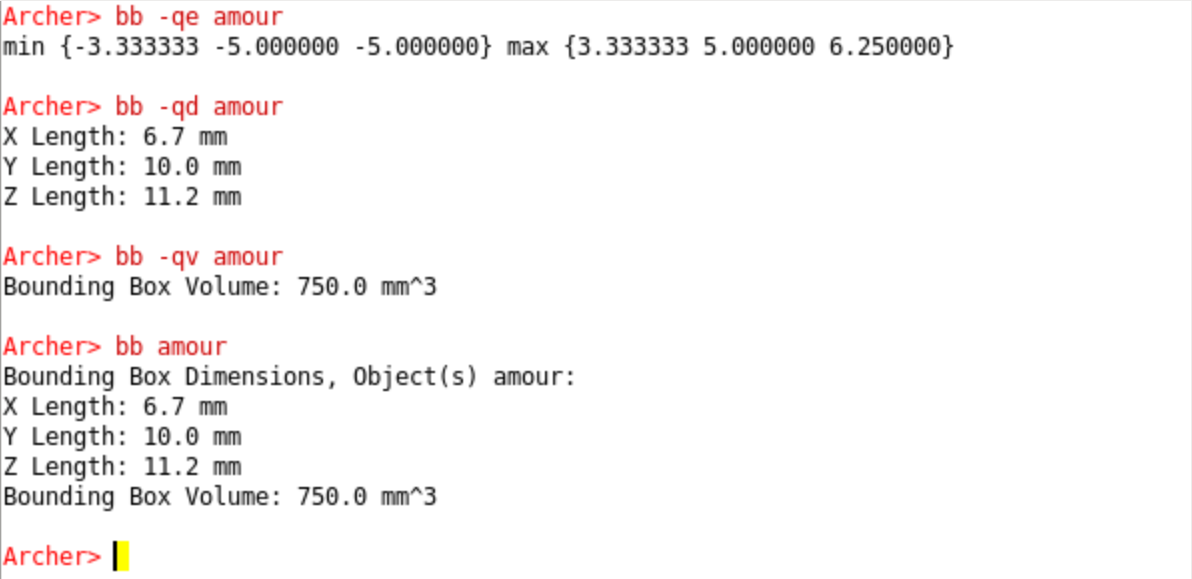
\includegraphics[trim=0.0cm 0.5cm 0.1cm 0.1cm, clip=true, totalheight=0.4\textheight]{Pictures/Bounding.png}
\caption[Testing the bounding box of the heart­-shape]{Testing the bounding box of the heart­-shape}
\label{Bounding}
\end{figure}

\clearpage

%---------------------------------------------------------------------------------------------------------------------

%---------------------------------------------------------------------------------------------------------------------
%				SECTION 4
%---------------------------------------------------------------------------------------------------------------------
\section{Plotting the wireframe of the heart­-shaped primitive}

\hspace{30} The   process   of   modeling   sometimes   warrants   the   preview   of   the   skeleton  
of   a   specific   set   of   objects.   To   test   that   the   wireframe   of   the   heart­-shaped  
primitive   is   working,   we   use   the   \textit{\textbf{draw}}[41]   command   in   BRL­-CAD.   The   \textit{\textbf{draw}}  
command   displays   objects   in   either   the   mged   or   archer   interfaces.   It   is  
synonymous   to   BRL­-CAD's   \textit{\textbf{e}}   command.   The   draw   command's   \textit{\textbf{-­C} (colour)}  
option   enables   the   user   to   specify   a   colour   that   overrides   all   other   previous  
colour specifications.  

\hspace{30} To   draw   the   wireframe   of   the   amour   object   using   white   wires,   we   run   the  
\textit{\textbf{“draw -­C 255/255/255 amour”}}   command.   The   image   in   Figure   4.4   below   shows  
the wireframe of amour with red iso­contours.  

\begin{figure}[htbp]
\centering
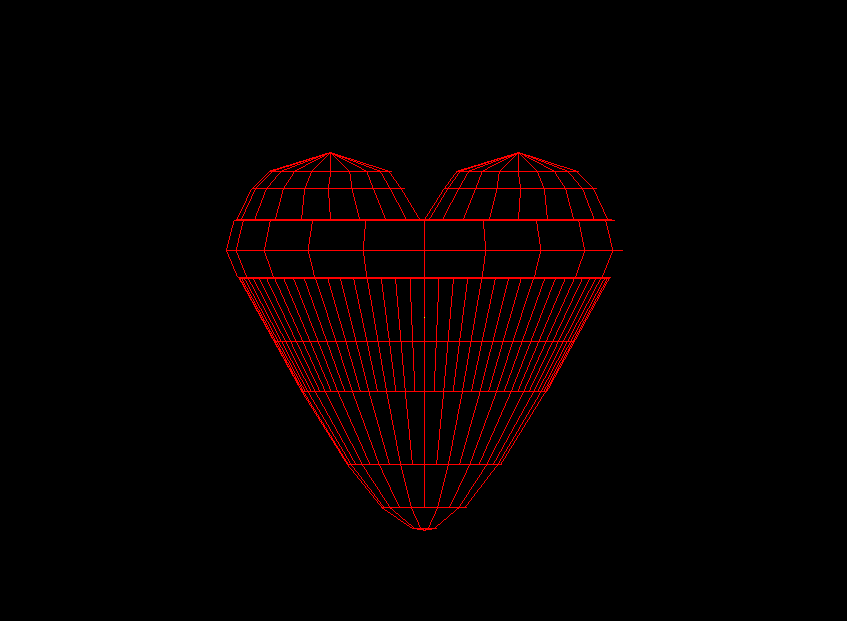
\includegraphics[trim=0.0cm 0.5cm 0.1cm 0.1cm, clip=true, totalheight=0.4\textheight]{Pictures/Wireframe.png}
\caption[Testing the wireframe of the heart­shaped primitive]{Testing the wireframe of the heart­shaped primitive}
\label{Wireframe}
\end{figure}

%---------------------------------------------------------------------------------------------------------------------

%---------------------------------------------------------------------------------------------------------------------
%				SECTION 5
%---------------------------------------------------------------------------------------------------------------------

\section{Ray tracing and surface representation of the heart-­shaped primitive}

\hspace{30} Ray­tracing   the   heart­-shaped   primitive   is   the   most   important   geometric  
property   because   the   others   lose their relevance without   BRL­-CAD's   capacity   to   render  
the   heart­-shaped   primitive.   A   major   difficulty   during   the   raytracing   of   the  
heart­-shaped   primitive   was   the   misunderstanding   that   the   sextic   equation   could  
be solved in radicals and only algebraic methods can be employed to solve it.  

\hspace{30} In   order   to   test   that   the   ray­tracing   property   of   the   heart­-shaped   primitive  
works, we use BRL-­CAD's \textit{\textbf{rt}}[42] command. The \textit{\textbf{rt}} command ray­traces a set
 of objects with the default option of \textit{\textbf{-­s50}}. Like other BRL­-CAD commands, it has various options.

\begin{itemize}
\item The \textit{\textbf{-a} (azimuth)} option enables the designer to specify the azimuth at which the rendered image will be created.  
\item The \textit{\textbf{-­e} (elevation)} option enables the designer to specify the elevation at which the rendered image should be created.  
\item The \textit{\textbf{-w} (width)} option enables the designer to specify the width of the rendered image.  
\item The \textit{\textbf{-­n} (height)} option enables the designer to specify the height of the rendered image.  
\item The \textit{\textbf{-­s} (size)} option enables the designer to specify the length of the rendered image (which is a square).  
\item The \textit{\textbf{-­C} (colour)} option enables the designer to specify the colour of the rendered image's background.  
\item The \textit{\textbf{-­o} (output)} option enables the designer to specify the name of the rendered image.
\end{itemize}

\clearpage
%----------------------------------------------------------------------------------------------------------------------

%----------------------------------------------------------------------------------------
%	SECTION 2
%----------------------------------------------------------------------------------------

\section{Main Section 2}

Sed ullamcorper quam eu nisl interdum at interdum enim egestas. Aliquam placerat justo sed lectus lobortis ut porta nisl porttitor. Vestibulum mi dolor, lacinia molestie gravida at, tempus vitae ligula. Donec eget quam sapien, in viverra eros. Donec pellentesque justo a massa fringilla non vestibulum metus vestibulum. Vestibulum in orci quis felis tempor lacinia. Vivamus ornare ultrices facilisis. Ut hendrerit volutpat vulputate. Morbi condimentum venenatis augue, id porta ipsum vulputate in. Curabitur luctus tempus justo. Vestibulum risus lectus, adipiscing nec condimentum quis, condimentum nec nisl. Aliquam dictum sagittis velit sed iaculis. Morbi tristique augue sit amet nulla pulvinar id facilisis ligula mollis. Nam elit libero, tincidunt ut aliquam at, molestie in quam. Aenean rhoncus vehicula hendrerit.
